\documentclass[nobib,nofonts]{tufte-handout}

%\geometry{showframe} % display margins for debugging page layout

%%% MF additions
\usepackage[nographicx, nohyperref, nosubcaption, nogb4e, nobiblatex]{../99-auxiliary-files/00-mypackages}
\usepackage{../99-auxiliary-files/00-mycommands}
\usepackage{../99-auxiliary-files/00-myenvironments}

\usepackage{titlesec}
\usepackage{etoolbox}
% \titleformat{\section}
% {\large\bfshape}{\thesection}{1em}{}

\setcounter{secnumdepth}{5}
\renewcommand\thesection{\arabic{section}}

% this length controls tha hanging indent for titles
% change the value according to your needs
\newlength\titleindent
\setlength\titleindent{0.7cm}

\pretocmd{\paragraph}{\stepcounter{subsection}}{}{}
\pretocmd{\subparagraph}{\stepcounter{subsubsection}}{}{}

\titleformat{\chapter}[block]
  {\normalfont\huge\bfseries}{}{0pt}{\hspace*{-\titleindent}}

\titleformat{\section}
  {\normalfont\Large\itshape}{\llap{\parbox{\titleindent}{\thesection\hfill}}}{0em}{}

\titleformat{\subsection}
  {\normalfont\itshape}{\llap{\parbox{\titleindent}{\thesubsection\hfill}}}{0em}{}

\titleformat{\subsubsection}
  {\normalfont\normalsize\itshape}{\llap{\parbox{\titleindent}{\thesubsubsection}}}{0em}{}

\titleformat{\paragraph}[runin]
  {\normalfont\normalsize\itshape}{}{-0.7cm}{}[\xspace \ \ \ \ ]

\titleformat{\subparagraph}[runin]
  {\normalfont\normalsize}{\llap{\parbox{\titleindent}{\thesubsubsection\hfill}}}{0em}{}

\titlespacing*{\chapter}{0pt}{0pt}{20pt}
\titlespacing*{\subsubsection}{0pt}{3.25ex plus 1ex minus .2ex}{1.5ex plus .2ex}
\titlespacing*{\paragraph}{0pt}{3.25ex plus 1ex minus .2ex}{0em}
\titlespacing*{\subparagraph}{0pt}{3.25ex plus 1ex minus .2ex}{0em}

\DefineNamedColor{named}{mygray2}{cmyk}{0.55,0.25,0.25,0.25}
\newcommand{\mygray}[1]{\textcolor{mygray2}{#1}}

%%% Tufte style
\usepackage{graphicx} % allow embedded images
  \setkeys{Gin}{width=\linewidth,totalheight=\textheight,keepaspectratio}
  \graphicspath{{graphics/}} % set of paths to search for images

\usepackage{fancyvrb} % extended verbatim environments
  \fvset{fontsize=\normalsize}% default font size for fancy-verbatim environments

% Standardize command font styles and environments
\newcommand{\doccmd}[1]{\texttt{\textbackslash#1}}% command name -- adds backslash automatically
\newcommand{\docopt}[1]{\ensuremath{\langle}\textrm{\textit{#1}}\ensuremath{\rangle}}% optional command argument
\newcommand{\docarg}[1]{\textrm{\textit{#1}}}% (required) command argument
\newcommand{\docenv}[1]{\textsf{#1}}% environment name
\newcommand{\docpkg}[1]{\texttt{#1}}% package name
\newcommand{\doccls}[1]{\texttt{#1}}% document class name
\newcommand{\docclsopt}[1]{\texttt{#1}}% document class option name
\newenvironment{docspec}{\begin{quote}\noindent}{\end{quote}}% command specification environment

%%%%%%%%%%%%%%%%%%%%%%%%%%%%%%%%%%%%%%%%%%%%%%%%%%

% \usepackage[sc,osf]{mathpazo}
% \linespread{1.05}



\title{Sets, relations, functions, and proofs}

\author[M.~Franke]{Michael Franke}

\date{} % without \date command, current date is supplied

\begin{document}

\maketitle

\begin{abstract}
\noindent
Basic notions of (na\"{i}ve) set theory; sets, elements, relations between and operations on
sets; relations and their properties; functions and their properties. Examples of informal
proofs: direct, indirect and counterexamples.
\end{abstract}

\section{Na\"{i}ve set theory}

\subsection{Sets, elements, universe}
\label{sec:sets}

A \emph{set} is a collection of entities. We use notation with curly braces ``$\set{\ldots}$''
to represent such a collection. If we have entities $a$ and $b$, examples of sets are:

\begin{multicols}{2}
  \begin{enumerate}[]
  \item $X = \set{a}$
  \item $Y = \set{a, b}$
  \end{enumerate}
\end{multicols}

\begin{marginfigure}
  \includegraphics{Cantor_set_definition.png}
  \caption{Passage first introducing the intuitive notion of a set from (the English
    translation of) Georg Cantor's \emph{Beiträge zur Begründung der transfiniten Mengenlehre}
    from 1915.}
\end{marginfigure}

\noindent The entity $a$ is an \emph{element} of $X$ and $Y$. We write this as $a \in X$ and $a \in
Y$. The entity $b$ is not an element of $X$. We write this as $b \not \in X$.

A set is individuated by the elements it contains. This means that the order of representation
of elements is irrelevant. For example, $\set{a,b} = \set{b,a}$. This also means that whenever
any two sets (however obtained) contain the same elements, they are identical. In other words,
for any two sets $X$ and $Y$ to be different, there has to be at least one element $x \in X$
such that $x \not \in Y$ or some $y \in Y$ such that $y \not \in X$.

It is possible for a set to have no element at all. This set is called the \emph{empty set} and
we refer to it with the symbol $\emptyset$.

Occasionally we might wish to specify the \emph{universe} $U$ of all entities which are under
consideration.\sidenote[][-0.75cm]{
  $U$ need not be a set itself; it can be something bigger. But that is best left aside here. The whole concept of a universe might seem confusing at first sight. It is possible not to deeply understand what it is good for in the greater scheme of things, and still understand everything of current relevance about na\"{i}ve set theory.
}
Any specification of a set is then implicitly restricted to entities in $U$.

\subsection{Ways of describing or defining sets}

Three main methods for describing or defining sets exist:
\begin{enumerate}
\item by listing elements
\item by characteristic property
\item by recursive definition
\end{enumerate}

\noindent The text above already gave examples for describing sets by \emph{listing
elements}. Sometimes we use notation ``\dots'' to indicate a range of elements when there is a
clear intuitive ordering relation among them. Or we use ``\dots'' to abbreviate the obvious
other members, even if there is no natural ordering. For example:

\begin{enumerate}[]
\item $X = \set{2, 4, 6, 8, \dots}$ \hfill \mygray{[set of even integers bigger than 0]}
\item $Y = \set{2, 4, 6, 8, \dots, 20}$ \hfill \mygray{[set of even integers no bigger than
    20]}
\item $Z = \set{\text{Russell}, \text{Wittgenstein}, \text{Frege}, \dots}$\sidenote{This would
  only be a good definition if the way to fill the ``$\dots$'' was absolutely clear.} \hfill {\mygray{[set of
    authors to read]}}
\end{enumerate}

To describe sets by a \emph{characteristic property} of its elements, we might write:

\begin{enumerate}[]
\item $X = \set{x \setbar \text{$x$ is an even integer}}$
\item $Y = \set{x \setbar \text{$x$ is an even integer no bigger than 20}}$
\item $Z = \set{x \setbar \text{$x$ is a famous logician}}$
\end{enumerate}

\noindent To narrow down a reference set explicitly, we would write:\sidenote{With a universe
  $U$ in place, we should read a description like
  \begin{align*}
    X & = \set{x \setbar \text{property of $x$}}\,, \ \  \text{as} \\
    X & = \set{x \in U \setbar \text{property of $x$}}\,.
  \end{align*}}

\begin{enumerate}[]
\item $X = \set{x \in \set{1, 2, 3, \dots} \setbar \text{$x$ is even}}$
\item $Y = \set{x \in \set{1, 2, 3, \dots, 20} \setbar \text{$x$ is even}}$
\item $Y = \set{x \in \set{y \setbar \text{$y$ is a logician}} \setbar \text{$x$ is famous}}$
\end{enumerate}

To describe sets by \emph{recursive definition}, we must:\sidenote{Recursive
  definitions are useful because they allow for easier proofs and easier further
  definitions. This will become clear when we look at a recursive definition of the formulas of
  a logical language, to which we will then assign a meaning by exploiting the original
  recursive definition (keyword: ``Tarski truth conditions'').}
\begin{enumerate}[(i)]
\item anchor the recursion
\item specify a recursion step
\item exclude elements untouched by anchor or recursive steps
\end{enumerate}
An example is the following definition of natural numbers:
\begin{enumerate}[(i)]
\item 0 is a natural number
\item if $n$ is a natural number, then so is $n+1$
\item nothing else is a natural number
\end{enumerate}
Another example is the definition of a simple formal language $\mathfrak{L}$. Unlike the
previous example, we here define a set of symbols:\sidenote{Examples
  of elements of $\mathfrak{L}$ by this definition are: ``three'', ``twenty minus three'',
  ``twenty minus three plus four''. Not an
  element of $\mathfrak{L}$ are ``minus three'', ``plus one two'', ``one plus minus two''.}
\begin{enumerate}
\item words for all natural numbers are elements of $\mathfrak{L}$ (e.g., ``one'', ``two'', \dots)
\item if $x, y \in \mathfrak{L}$, then so are the strings:
  \begin{multicols}{2}
    \begin{itemize}[]
    \item ``$x$ plus $y$''
    \item ``$x$ minus $y$''
    \end{itemize}
  \end{multicols}
\item no string which is not constructible by this procedure is in $\mathfrak{L}$
\end{enumerate}

\subsection{Important numerical sets to be familiar with}

Important sets to be familiar with are:\sidenote{Notice the commonly used ``double-stroke notation'' for the capital letters used to refer to these special sets.}
\begin{enumerate}[]
\item $\mathbb{N} = \set{0, 1,2,3, \dots}$ \hfill \mygray{[set of natural numbers]}
\item $\mathbb{Z} = \set{\dots, -2, -1, 0, 1, 2, \dots}$ \hfill \mygray{[set of integers]}
\item $\mathbb{Q} = \set{\nicefrac{p}{q} \setbar p \in \mathbb{Z}, q \in \mathbb{N} \setminus \set{0}}$ \hfill \mygray{[set of rational
    numbers]}
\item $\mathbb{R} = \set{\pi, 0, e, \dots}$ \hfill \mygray{[set of real numbers]}
\end{enumerate}

\subsection{Cardinality}

The number of elements in a set is called its \emph{cardinality}.
We write $\card{X}$ for the cardinality of $X$. The cardinality of $X$ can be infinite.
We then write $\card{X} = \infty$ and say that $X$ is an infinite set.\sidenote{Actually, infinite sets can have different cardinalities, so that writing $\card{X} = \infty$ could be misleading. For example, $\card{\mathbb{N}} = \card{\mathbb{Q}} < \card{\mathbb{R}}$. But this is not important for us at the moment.}
If $X$ is not an infinite set, it is called a \emph{finite set}.
Examples:
\begin{align*}
  &\card{\set{a}} = 1 && \card{\set{a,b}} = 2 \\
  & \card{\es} = 0    && \card{\set{2,4,6,8 \dots}} = \infty
\end{align*}

\subsection{Relations between sets}

A set $Y$ can contain another set $X$. Inversely, a set $X$ can be an element of another set
$Y$. We then write $X \in Y$. For example:
\begin{enumerate}[]
  \item $X = \set{a,b}$ 
  \item $Y = \set{c, d, X} = \set{c, d, \set{a,b}}$
\end{enumerate}
It is important to note that $\set{a,b} \in Y$ but $a \not \in Y$. 

If all of the elements of $X$ are also in $Y$, we say that $X$ is a \emph{subset} of $Y$, or
that $Y$ is a \emph{superset} of $X$, and we write $X \subseteq Y$. If $X \subseteq Y$ and
there is at least one element in $Y$ which is not in $X$, we say that $X$ is a \emph{proper
  subset} of $Y$, or that $Y$ is a \emph{proper superset} of $X$, and we write $X \subset
Y$.
If $X$ is not a (proper) subset of $Y$, we write $X \not \subseteq Y$ ($X \not \subset
Y$). Some examples:
\begin{multicols}{2}
  \begin{enumerate}[]
  \item $\set{a,b} \subseteq \set{a,b,c}$
  \item $\set{a,b} \not \subseteq \set{a,c}$
  \item $\set{a,b} \subset \set{a,b,c}$
  \item $\set{a,b} \not \subset \set{a,b}$
  \end{enumerate}
\end{multicols}

\subsection{Operations on sets}

Operations on sets take one or several sets as input and return another set.
We consider here the power set operation and different kinds of logical operations.

The \emph{power set} $\pow{X}$ of $X$ is the set of all subsets of $X$:
\begin{align*}
  \pow{X} = \set{Y \setbar Y \subseteq X}
\end{align*}
If $X$ is finite, the cardinality of $\pow{X}$ is $2^{\card{X}}$.\sidenote{This is because we
  decide $\card{X}$ times whether to include an element or not; so we collect all outcomes of
  $\card{X}$ binary decisions.} For example:
\begin{multicols}{2}
  \begin{enumerate}[]
  \item $X = \set{a,b}$
  \item $\pow{X} = \set{\emptyset, \set{a}, \set{b}, \set{a,b}}$
  \item $\card{X} = 2$
  \item $\card{\pow{X}} = 2^2 = 4$
  \end{enumerate}
\end{multicols}


\begin{marginfigure}[2cm]
  \includegraphics{set_operations.png}
  \caption{Venn diagrams of set operations.}
\end{marginfigure}

The following operations on sets correspond to logical operators (\emph{and}, \emph{or}, \emph{not}).
For any sets $X$ and $Y$:
\begin{enumerate}[]
\item $X \cap Y = \set{z \setbar z \in X \text{ and } z \in Y}$ \hfill \mygray{[intersection]}
\item $X \cup Y = \set{z \setbar z \in X \text{ or } z \in Y}$ \hfill \mygray{[union]}
\item $X \setminus Y = \set{z \setbar z \in X \text{ and } z \not \in Y}$ \hfill
  \mygray{[difference]}
\item $\overline{X} = \set{z \in U \setbar z \not \in X }$ \hfill
  \mygray{[complement\sidenote{We need an explicit universe to interpret the complement operation.}]}
\end{enumerate}
Here are some examples:
\begin{multicols}{2}
  \begin{enumerate}[]
  \item $X = \set{a,b,c}$
  \item $Y = \set{b,c,d}$
  \item $X \cap Y = \set{b, c}$
  \item $X \cup Y = \set{a, b, c, d}$
  \item $X \setminus Y = \set{a}$
  \item $Y \setminus X = \set{d}$
  \end{enumerate}
\end{multicols}

\begin{marginfigure}
  \includegraphics{set_theory_laws.png}
  \caption{Some facts. NB: The complement of set $X$ is written as $X'$ in this list.}
  \label{fig:facts-of-settheory}
\end{marginfigure}

A number of facts follows from the definitions so far.
Some are shown in Figure~\ref{fig:facts-of-settheory}.
To conclusively show that something follows from a definition, we need the concept of a \emph{proof}, the topic of the next section.

\bigskip
\noindent \colorbox{mygray}{\centering
  \begin{minipage}{1.0\textwidth}

    \begin{exercise}
      Provide a natural language paraphrase for each of the following sets:
      \begin{enumerate}[a.]
        \item $A = \set{5, 7, 9, 11, 13, \dots}$
        \item $B = \mathbb{N} \setminus A$
        \item $C = \set{c \in \mathbb{Z} \mid -2 \le c \le 2}$
        \item $D = \mathbb{N} \cap \overline{C}$
      \end{enumerate}
    \end{exercise}

    \begin{exercise}
      Let's assume the following definitions (assuming that the universe is $U = X \cup Y \cup Z$):
      \begin{align*}
        X & = \set{a, b, c, d} \\
        Y & = \set{y \mid y \text{ is a vowel}} = \set{a, e, i, o, u} \\
        Z & = \set{z \mid z \text{ is an even natural number smaller than 5}}
      \end{align*}
      Write out the results of the following set operations:
      \begin{multicols}{3}
      \begin{enumerate}[a.]
        \item $X \cap Y$
        \item $X \cup Y$
        \item $X \setminus Y$
        \item $Y \setminus Z$
        \item $Y \setminus Y$
        \item $X \cap \overline{X}$
      \end{enumerate}
    \end{multicols}
    \end{exercise}

    \begin{exercise}
      For each of the following statements, determine whether it is true or false, using the sets $X$, $Y$ and $Z$ as defined above:
      \begin{multicols}{3}
        \begin{enumerate}[a.]
          \item $X \subset Y$
          \item $Y \in X$
          \item $X \cap Y \subseteq X$
          \item $\card{X} = \card{Y}$
          \item $X \cup Z \subseteq X$
          \item $X \cap Y \not \subset X$
        \end{enumerate}
      \end{multicols}

    \end{exercise}

  \end{minipage}
}

\newpage

\section{Proofs}

\subsection{Formal vs.~informal proofs}

There are two general kinds of proofs.
\emph{Formal proofs} are rigid rule-based derivations operating on a formal language in a specific proof system.\sidenote{Formal proofs will be dealt with later in the context of a logic.}
\emph{Informal proofs}, if done well, follow the structure of a formal proof but only describe the gist of it in more comprehensible language, usually a mix of natural language, specialized jargon and mathematical notation.
When we speak of proofs from here on, think: informal proof.

\subsection{Why proofs?}

Nothing can be known for certain, except mathematical-logical truth.\sidenote{This is a strategically bold claim to clearly emphasize the significance of mathematical-logical knowledge. Please feel highly provoked and intrigued. Please push back, question and doubt!}
Proofs are the anchors of infallible, necessarily true knowledge.
A proposition which has a valid proof must necessarily be true (in the system of logic and given the assumptions used to prove it).
Therefore, proofs are the foundation of the only unshakable knowledge humankind is capable of.

\subsection{Proof strategies}

There are different kinds of proof strategies, which can be applied in different kinds of situations.
Here we will look at the following four proof strategies:

\begin{enumerate}[(i)]
  \item refutation by counterexample
  \item direct proof
  \item indirect proof
  \item inductive proof
\end{enumerate}

\paragraph{Refutation by counterexample.}

The perhaps easiest kind of proof is \emph{refutation by counterexample}.
It can be used to prove the falsety of a claim that some general law is true.
Below is an example.
The claim in Proposition~\ref{prop:refut-count-1} is a general statement about any two sets $X$ and $Y$.
But it is false.
We can show that it is false by giving just a single instance of $X$ and $Y$ which refutes
it.\sidenote[][-0.75cm]{We should not confuse mathematical statements with statistical
  generalizations, which might tolerate exceptions. It is irrelevant that there are other pairs
  of sets $X$ and $Y$ for which the claim would be true, such as: $X = \set{a}$,
  $Y=\set{a, \set{a}}$.}

\begin{proposition}
  \label{prop:refut-count-1}
  The following claim is false: For any sets $X$ and $Y$, if $X \in Y$, then all the elements of $X$ are also elements of $Y$.
\end{proposition}

\begin{proof}
  A counterexample to the claim in question is given by the following two sets:
  \begin{enumerate}[]
    \item $X = \set{a,b}$
    \item $Y = \set{c, d, X} = \set{c, d, \set{a,b}}$
  \end{enumerate}
  Although $X \in Y$ and $a \in X$, it is not true that $a \in Y$.\sidenote{To mark the end of a proof, we here use the symbol $\Box$. Another common end-of-proof notation is ``QED'', short for \emph{quod erat demonstrandum} (what was to be shown).}
\end{proof}

Here is a second example.

\begin{proposition}
  The following claim is false: If $X \cup Y \neq \es$, then $X \cap Y \neq \es$.
\end{proposition}

\begin{proof}
  A counterexample is $X = \set{a}$ and $Y=\set{b}$, because clearly $\set{a} \cup \set{b} = \set{a,b} \neq \es$, but $\set{a} \cap \set{b} = \es$.
\end{proof}

\paragraph{Direct proof.}

A direct proof of a statement proceeds by unraveling definitions and axioms until what needs to be shown is plain to see.

\begin{proposition}
  \label{prop:emptyset-subset-of-any-X}
  For any $X$, $\emptyset \subseteq X$.
\end{proposition}

\begin{proof}
  Consider an arbitrary set $X$. For a set $Y$ be a subset of $X$, it is required that all elements of $Y$ are also in $X$. Another way of putting this is that there cannot be a single element $y \in Y$ for which $y \not \in X$. Since the empty set contains no elements at all, there cannot be any element in it, which is not also in $X$.
\end{proof}

If the statement to be proven is a conditional with \emph{if} and \emph{then}, then the direct proof may also use the content of the \emph{if} part as part of its derivation.

\begin{proposition}
  If $X \cap Y \neq \es$, then $\card{X \cup Y} > 0$.
\end{proposition}

\begin{proof}
  Suppose that $X \cap Y \neq \es$. This means that there must be at least one element $z$ that
  is in both $X$ and $Y$. But then the number of elements that are in either $X$ or $Y$ must be
  at least one and so bigger than zero.
\end{proof}

\paragraph{Indirect proof.}

Direct proofs can sometimes be hard (even impossible), while a different strategy, namely an indirect proof is much easier.
To indirectly prove a claim, we assume the logical opposite of what needs to be shown and derive from it a contradiction.
This strategy is therefore also called \emph{reductio ad absurdum} or \emph{proof by refutation}.
This is best demonstrated with a series of examples.

Let us start with an indirect proof for Proposition~\ref{prop:emptyset-subset-of-any-X}, for which we had a direct proof above already.
The proposition is that: For any $X$, $\es \subseteq X$.

\begin{proof}
  Assume that there is an $X$ for which $\es \not \subseteq X$.\sidenote{Here is the \emph{reductio} assumption. We simply assume the opposite of what we want to show.} Then there must be an element in $\es$ which is not in $X$. But there are no elements in $\es$. So, we have a contradiction.\sidenote{We derive a contradiction from the assumption that what needed to be shown is false. Hence, what needed to be shown must be true.}
\end{proof}

Here is another example.

\begin{proposition}
  There can be at most one empty set.
\end{proposition}

\begin{proof}
  Suppose that there are two empty sets.\sidenote{This is the reductio assumption that the \emph{opposite} of
    what we want to show is true.} Call them $\es_1$ and $\es_2$. Sets are
  individuated by the elements that they contain. So for $\es_1$ and $\es_2$ to be different,
  there needs to be an entity $x$ such that $x \in \es_1$ and $x \not \in \es_2$ or
  $x \in \es_2$ and $x \not \in \es_1$. But since both $\es_1$ and $\es_2$ are empty, there
  cannot be such an entity $x$. Hence, there cannot be two empty sets.
\end{proof}

And another example, this time for a conditional statement.
Notice that now the \emph{reductio} assumption is slightly more complicated.

\begin{proposition}
  If $X \subseteq Y$ and $Y \subseteq X$, then $X = Y$.
\end{proposition}
\begin{proof}
  Let us assume that $X \subseteq Y$ and $Y \subseteq X$ and also that $X \neq Y$.\sidenote{We assume that the content of the \emph{if}-statement is true and we also assume, towards deriving a contradiction, that the content of the \emph{then}-statement is false, contrary to what the proposition says.}
  The latter means that there must be some element $x \in X$ such that $x \not \in Y$ or some element $y \in Y$ such that $y \not \in X$.
  If there is an $x \in X$ with $x \not \in Y$, it cannot be that $X \subseteq Y$. If there is an $y \in Y$ with $y \not \in X$, it cannot be that $Y \subseteq X$. This is a contradiction to our initial assumption.
\end{proof}

\paragraph{Inductive proof.}
There are also inductive proofs.
These are more complicated, as they consist of three steps: the inductive base, the inductive assumption and the inductive step.

Inductive proofs are often useful in connection with recursive definitions.
Let us consider a very simple example first.
We use the following recursive definition of a set $\mathcal{F}$ of (flowery) strings:

\begin{enumerate}
  \item \textbf{anchor:} the symbol ``*'' is part of $\mathcal{F}$
  \item \textbf{step:} if $f \in \mathcal{F}$, then so is ``(f)''
  \item \textbf{exhaustion:} nothing else is in $\mathcal{F}$
\end{enumerate}


\begin{proposition}
  Each $f \in \mathcal{F}$ contains the exact same number of opening and closing parentheses.
\end{proposition}

\begin{proof}
  The inductive proof is over the number $n$ of opening parentheses.

  \emph{Inductive base.}
  Any element in $\mathcal{F}$ which has no opening parentheses is necessarily added to $\mathcal{F}$ by the recursive anchor. But since the recursive anchor introduces neither opening nor closing parentheses, the number of opening and closing parentheses for $n=0$ is equal.

  \emph{Inductive assumption.} We assume that any string $f \in \mathcal{F}$ with $n = k-1$ opening parentheses has the same number of opening and closing parentheses.

  \emph{Inductive step.}
  We now need to show that a string $f \in \mathcal{F}$ with $n=k$ opening parentheses also has $n=k$ closing parentheses.
  Indeed, the only way in which $f$ can have $n>0$ opening parentheses is by application of the recursive step.
  Therefore, $f$ must be of the form $f = \text{``(g)''}$ where string $g \in \mathcal{F}$ has $k-1$ opening parentheses.
  By inductive assumption, $g$ has the same amount of opening and closing parentheses.
  But since $f = \text{``(g)''}$, and so exactly one parenthesis of each type is added to $g$, $f$ must have an equal number of parentheses, too.
\end{proof}

Here is another, more difficult application of an inductive proof.

\begin{proposition}
  The cardinality of the power set of finite set $X$ is $\card{\pow{X}} = 2^{\card{X}}$.
\end{proposition}

\begin{proof}
  The inductive proof is over the cardinality of set $X$.\\
  \emph{Inductive base.} If $\card{X} = 0$, we know that $X = \emptyset$, so that $\pow{X} = \set{\emptyset}$. The cardinality of $\set{\emptyset}$ is indeed $2^{\card{X}} = 2^{0} = 1$.\sidenote{Though strictly speaking unnecessary, we might also check the case of $n=1$ just to be sure: If $\card{X} = 1$, we know that $X = \set{x}$, so that $\pow{X} = \set{\emptyset, \set{x}}$, the cardinality of which is $2^{\card{X}} = 2$. } \\
  \emph{Inductive assumption.} Assume that the claim is true for any set with cardinality of at most $n > 0$.\\
  \emph{Inductive step.} We need to show that the claim is true for any set $X$ with $\card{X} = n$, given the inductive assumption.
  Let $X$ be an arbitrary set with $\card{X} = n$.
  Let $x \in X$ and $Y = X \setminus \set{x}$. By inductive assumption, $\card{\pow{Y}} = 2^{\card{Y}}$.
  The power set of $X$ contains all sets in the power set of $Y$.
  It additionally also contains a version of each element in $\pow{Y}$ that also contains $x$.\sidenote{This may be intuitively clear, but it might also be proven (as a so-called \emph{lemma}). It is in this sense that these proofs are all informal: they do not spell out each and every piece of the derivation which may be plausible enough to be left out.}
  But that means that the cardinality of $\pow{X}$ is $\card{\pow{X}} = 2 \times \card{\pow{Y}} = 2 \times 2^{{n-1}} = 2^{n}$.
\end{proof}

\bigskip
\noindent \colorbox{mygray}{\centering
  \begin{minipage}{1.0\textwidth}

    \begin{exercise}
      Show that $X \cap \overline{X} = \emptyset$ for any set $X$.
    \end{exercise}

    \begin{exercise}
      Previously, in Section~1, we defined a simple formal language $\mathfrak{L}$ recursively as the smallest set such that:
      \begin{enumerate}
        \item all words for natural numbers, i.e., ``one'', ``two'', \dots, are in $\mathfrak{L}$
        \item if $x, y \in \mathfrak{L}$, then so are the strings:
        \begin{multicols}{2}
          \begin{itemize}[]
            \item ``$x$ plus $y$''
            \item ``$x$ minus $y$''
          \end{itemize}
        \end{multicols}
      \end{enumerate}
      Prove the following statement with an inductive proof strategy: No element of $\mathfrak{L}$ is a string that contains the work ``bread.''
    \end{exercise}

    \begin{exercise}
      Using the set $\mathfrak{L}$ as constructed above, use an indirect proof to show that the length of elements of $\mathfrak{L}$ is unbounded (i.e., for any $x \in \mathfrak{L}$ there is a $y \in \mathfrak{L}$ such that $y$ has strictly more words than $x$.)
    \end{exercise}
  \end{minipage}
}

\newpage

\section{Relations}

While sets capture (what philosophers call) the \emph{extensional meaning} of a property like ``$x$ is red'', in terms of the set of all red objects (from a relevant universe), a relation captures the extensional meaning of expressions like ``$x$ is in love with $y$''.

\subsection{Tuples, Cartesian products}

Recall that sets are individuated by their elements, but not by the way in which these elements
are picked out or arranged.
In particular $\set{x,y} = \set{y,x}$.
An \emph{ordered pair}, written as $\tuple{x,y}$, is sensitive to ordering information, so that:
$\tuple{x,y} \neq \tuple{y,x}$.
We generalize the notion of an ordered pair to an \emph{$n$-tuple}, written as $\tuple{x_1, x_2, \dots, x_n}$.\sidenote{We can allow for $1$-tuples as well and think of them as just the element itself, i.e., $\tuple{a} = a$.}\sidenote{$3$-tuples are also called triples; $4$-tuples quadruples; $5$-tuples quintuples \dots}
An $n$-tuple contains more information than the set of elements in that $n$-tuple. For example, we might be interested in the unordered set of cities that Hans visited last summer:
\begin{align*}
  \set{x \setbar \text{$x$ is a city Hans
      visited last summer}} = \set{\text{London}, \text{Paris}, \text{Berlin}}
\end{align*}
or we might be interested in the cities that Hans visited in the order in
which he actually visited them:
\begin{align*}
  \tuple{\text{Berlin}, \text{London}, \text{Berlin}, \text{Paris}}
\end{align*}
The set does not give us information about the order, but also does not contain duplicates.
The tuple does.


The \emph{Cartesian product} of sets $X_1$, $X_2$, \dots, $X_n$ is the set of all $n$-tuples
$\tuple{x_1, x_2, \dots, x_n}$ such that $x_i$ is an element from set $X_i$:\sidenote{If we identify 1-tuples with the single element itself (see sidenote above), the Cartesian product of a single set $X$ is $X$ itself: $\set{\tuple{x} \setbar x \in X} = \set{x \setbar x \in X} = X$. }
\begin{align*}
  X_1 \times X_2 \times \ldots \times X_n  = \set{\tuple{x_1, x_2,
  \dots, x_n} \setbar x_1 \in X_1, x_2 \in X_2, \dots, x_n \in X_n}
\end{align*}
The sets forming a Cartesian product need not be different from each other.
Here are some examples for sets $X = \set{a,b}$ and $Y = \set{c,d}$:
\begin{enumerate}[]
  \item $X \times Y = \set{\tuple{a,c}, \tuple{a,d}, \tuple{b,c}, \tuple{b,d}}$
  \item $X \times X = \set{\tuple{a,a}, \tuple{a,b}, \tuple{b,a}, \tuple{b,b}}$
  \item $X \times X \times Y = \{\tuple{a,a,c}, \tuple{a,b,c}, \tuple{b,a,c}, \tuple{b,b,c},$
    \item \ \ \ \ \ \ \ \ $\tuple{a,a,d}, \tuple{a,b,d}, \tuple{b,a,d}, \tuple{b,b,d}\}$
\end{enumerate}

The $n$-place Cartesian product with the same set $X$ can also be written as $X^{n}$:\sidenote{For example the set $\mathds{R}^{3}$ is a three dimensional vector space. Numerical tuples, like the elements of $\mathds{R}^{3}$ are \textit{vectors}.}
    \begin{align*}
      \underbrace{X \times X \times \dots \times X} _{n \text{ times }}= X^{n}
    \end{align*}

\subsection{Relations}

An \emph{$n$-place relation} $R$ is a set of $n$-tuples
$R \subseteq X_1 \times \dots \times X_n$.\sidenote{Instead of ``$n$-place'' we might also say
  ``$n$-ary'' and speak of the \emph{arity} of a relation.}\sidenote{A 1-place relation on set
  $X$ is just a subset of $X$; a 2-place relation is called binary relation; a 3-place relation
  is called ternary relation; \dots}
For example, consider the set of people $P = \set{j,m,s}$ of John, Mary and Sue and the binary relation $L \subseteq P \times P$ which encodes who loves whom:
\begin{align*}
  L & = \set{\tuple{x,y} \in P \times P \setbar \text{$x$ loves $y$}}
\end{align*}
Suppose we live in a world in which these are the facts:
\begin{align*}
  L  & = \set{\tuple{j,j}, \tuple{j,s}, \tuple{m,s}, \tuple{s,m}} \subset P \times P
\end{align*}
\noindent We can visualize relation $L$ in a diagram, like shown in Figure~\ref{fig:relationL}, where we
draw elements as dots (possibly with labels) and where we draw an arrow from element $x$ to
element $y$ whenever $\tuple{x,y}$ is part of the relation.
\begin{marginfigure}
  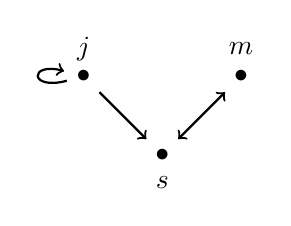
\begin{tikzpicture}

  \node (j) at (0,0)   {$\bullet$};

  \node (m) at (2,0)   {$\bullet$};

  \node (s) at (1,-1)  {$\bullet$};

  \node at (0,0.35)   {$j$};

  \node at (2,0.35)   {$m$};

  \node at (1,-1.35)   {$s$};

  % Arrows
  \path[thick,-to] (j) edge [loop left] (j);
  \draw[->, thick]  (j) -- (s);
  \draw[<->, thick] (m) -- (s);

\end{tikzpicture}
\caption{Diagram of relation $L$.}
\label{fig:relationL}
\end{marginfigure}

Another example is the binary relation ``$n_1$ is the predecessor of $n_2$'' on the set $\mathds{N}$ of natural numbers.
The predecessor relation $P \subseteq \mathds{N} \times \mathds{N}$, shown in Figure~\ref{fig:successor}, is defined as:
\begin{align*}
  P = \set{\tuple{0,1}, \tuple{1,2}, \tuple{2,3}, \dots}
\end{align*}
\begin{marginfigure}
  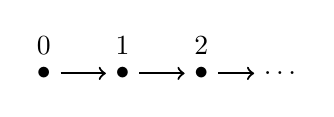
\begin{tikzpicture}

  \node (0) at (0,0)   {$\bullet$};
  \node (1) at (1,0)   {$\bullet$};
  \node (2) at (2,0)   {$\bullet$};
  \node (3) at (3,0)   {$\dots$};

  \node () at (0,0.35)   {0};
  \node () at (1,0.35)   {1};
  \node () at (2,0.35)   {2};
  \node () at (3,0.35)   {};

  % Arrows
  \draw[->, thick]  (0) -- (1);
  \draw[->, thick]  (1) -- (2);
  \draw[->, thick]  (2) -- (3);

\end{tikzpicture}
\caption{The predecessor relation on $\mathds{N}$.}
\label{fig:successor}
\end{marginfigure}


For a binary relation $R\subseteq X \times Y$, there are several shortcut notations to express the same content as when we write ``$\tuple{x,y} \in R$'':
\begin{enumerate}
\item[] \emph{prefix notation}: $Rxy$
\item[] \emph{infix notation}: $xRy$
\item[] \emph{postfix notation}: $xyR$
\end{enumerate}
From here on we will predominantly use prefix notation, except for known mathematical relations like $\le$ or $=$.

If $R \subseteq X \times Y$ is a binary relation, the \emph{domain} of $R$ is
\begin{align*}
  \text{dom}(R) = \set{x \in X \setbar \text{there is some $y \in Y$ with } Rxy}
\end{align*}
The \emph{range} of $R$ is
\begin{align*}
  \text{range}(R) = \set{y \in Y \setbar \text{there is some $x \in X$ with } Rxy}
\end{align*}
The \emph{negation} of $n$-place relation $R \subseteq X_1 \times \dots \times X_n$ is
\begin{align*}
  \overline{R} = (X_1 \times \dots \times X_n) \setminus R
\end{align*}
The \emph{convervse} of $n$-place relation $R \subseteq X_1 \times \dots \times X_n$ is
\begin{align*}
  R^{-1} = \set{\tuple{y,x} \setbar Rxy}
\end{align*}

\begin{claim}
  The following is false: If $R \subseteq X \times X$, then $\text{dom}(R) = \text{range}(R)$.
\end{claim}

\begin{proof}
A counterexample is $L' = L \setminus \set{\tuple{j,j}}$, with $L$ being the ``love relation'' introduced
above in Figure~\ref{fig:relationL}. Notice that: $L = \set{\tuple{j,j}, \tuple{j,s},
  \tuple{m,s}, \tuple{s,m}}$ and so $L' = \set{\tuple{j,s}, \tuple{m,s},
  \tuple{s,m}}$. According to $L'$ everybody loves someone so $\text{dom}(L') = \set{j,m,s}$,
but nobody loves John, so $j \not \in \text{range}(L') = \set{m,s}$.
\end{proof}


\subsection{Properties of binary relations}

Binary relation $R \subseteq X \times X$ is\sidenote{In definitions like these, we often write ``iff'' which can be read as ``if and only if'' or ``exactly if''.}
\begin{enumerate}
\item[] \emph{reflexive} iff $Rxx$ for all $x \in X$
\item[] \emph{irreflexive} iff $Rxx$ for no $x \in X$
\item[] \emph{symmetric} iff for all $x,y \in X$ if $Rxy$ then also $Ryx$
\item[] \emph{asymmetric} iff for no $x,y \in X$ both $Rxy$ and $Ryx$
\item[] \emph{anti-symmetric} iff for all $x,y \in X$ if $Rxy$ and $Ryx$, then $x = y$
\item[] \emph{transitive} iff for all $x,y \in X$ if $Rxy$ and $Ryz$, then also $Rxz$
\item[] \emph{intransitive} iff for all $x,y \in X$ if $Rxy$ and $Ryz$, then not $Rxz$
\item[] \emph{connected} iff for all $x,y \in X$ either $Rxy$ or $Ryx$ or $x = y$
\end{enumerate}

The relation $L$ in Figure~\ref{fig:relationL} does not have any of the properties above.
For example, it is not reflexive because there is an element, namely $m$, for which $Lmm$ is false.
It is also not irreflexive because there is an element, namely $j$, for which $Ljj$ is true.
It is not transitive, because although $Ljs$ and $Lsm$ it is not the case that $Ljm$.

The relation ``$n_1$ is the predecessor of $n_2$'' from Figure~\ref{fig:successor} is
irreflexive, asymmetric and intransitive. It is intransitive, because whenever $x$ is the
predecessor of $y$ we have $x + 1= y$, and whenever $y$ is the predecessor of $z$ we have
$y + 1 = z$. But then $x + 2= z$, so $x$ is not the predecessor of $z$.

\begin{proposition}
  \label{prop:proof-reflexive-range}
  If $R \subseteq X \times X$ is reflexive, then $\text{dom}(R) = \text{range}(R)$.
\end{proposition}

\begin{proof}
  Let $R \subseteq X \times X$ be reflexive and assume towards contradiction that $\text{dom}(R) \neq \text{range}(R)$. The latter means that there is either an
  $x \in \text{dom}(R)$ with $x \not \in \text{range}(R)$, or that there is $x \not \in
  \text{dom}(R)$ with $x \in \text{range}(R)$. But if we take an arbitrary $x \in X$, then by
  reflexivity $Rxx$. So $x \in \text{dom}(R)$ and $x \in \text{range}(R)$, which contradicts
  our assumption.
\end{proof}

\begin{proposition}
  If $R \subseteq X \times X$ is asymmetric, it is also irreflexive.
\end{proposition}

\begin{proof}
  If $R \subseteq X \times X$ is not irreflexive, then there is at least one $x^* \in X$ such
  that $Rx^*x^*$. But then there is also a pair $x,y \in X$ (namely with $x=x^*$ and $y = x^*$)
  such that $Rxy$ and $Ryx$. So $R$ is not asymmetric.\sidenote{This is a \emph{proof by
      contraposition}. To show that ``if $A$, then $B$'' we show that ``if not $B$, then not
    $A$''. This is justified because $p \leftarrow q$ and $\neg q \rightarrow \neg p$ are logically equivalent in propositional logic (as we will learn later).}
\end{proof}

\noindent Binary relation $R \subseteq X \times X$ is an \emph{equivalence relation} iff $R$ is reflexive,
symmetric and transitive. Equivalence relations are interesting because they cluster elements
by some criterion of sameness. Whence also the name. Given appropriate domains, the following
are examples of equivalence relations:
\begin{enumerate}
\item[] \dots and \dots have the same shoe size
\item[] \dots and \dots are born in the same year
\item[] \dots and \dots have the same color (see Figure~\ref{fig:equivRel})
\item[] \dots and \dots have the same cardinality
\end{enumerate}


\begin{figure*}
  \includegraphics[width = 0.7\textwidth]{equivalence_relation.png}
  \caption{Example of an equivalence relation based on property ``\dots and \dots have the same
  color''.}
  \label{fig:equivRel}
\end{figure*}

\noindent Based on different properties of relations, we can also define various notions of
``ordering''. Binary relation $R \subseteq X \times X$ is a
\begin{enumerate}
\item[] \emph{partial weak order} iff $R$ is reflexive, anti-symmetric and transitive \\
  \hfill \mygray{[example: relation ``$\subseteq$'' on $\pow{Y}$]}
\item[] \emph{partial strict order} iff $R$ is irreflexive, asymmetric and transitive \\
  \hfill \mygray{[example: relation ``$\subset$'' on $\pow{Y}$]}
\item[] \emph{linear weak order} iff $R$ is a partial weak order and connected \\
  \hfill \mygray{[example: relation ``$\le$'' on $\mathds{N}$]}
\item[] \emph{linear strict order} iff $R$ is a partial strict order and connected \\
  \hfill \mygray{[example: relation ``$<$'' on $\mathds{N}$]}
\end{enumerate}


\bigskip
\noindent \colorbox{mygray}{\centering
  \begin{minipage}{1.0\textwidth}

    \begin{exercise}
      Which proof strategy is used in the proof of Proposition~\ref{prop:proof-reflexive-range}?
    \end{exercise}

    \begin{exercise}
      Which properties do the following binary relations, expressed here in natural language, on the set of all human beings have?
      \begin{multicols}{2}
      \begin{enumerate}[a.]
        \item $x$ is taller than $y$
        % \item $x$ is smaller than $y$
        \item $x$ is the same person as $y$
        % \item $x$ admires $y$
        \item $x$ is the father of $y$
        \item $x$ has the same first name as $y$
      \end{enumerate}
    \end{multicols}
    \end{exercise}

    \begin{exercise}
      Consider the set $\mathds{N} = \set{0, 1, 2, \dots}$ of natural numbers and the binary relation $R \subseteq \mathds{N} \times \mathds{N}$ defined as follows:
      \begin{align*}
        R = \set{\tuple{x,y} \mid x, y \in \mathds{N} \text{ and } y = x^{2}}
      \end{align*}
      Which properties does $R$ have? Is $R$ a partial weak/strict order? Is it a linear weak/strict order? Is it an equivalence relation?
    \end{exercise}

  \end{minipage}
}

\newpage

\section{Functions}

\begin{marginfigure}
  \includegraphics[]{function_example.png}
  \caption{Example of function corresponding to description ``the height of $x$''.}
  \label{fig:function_ex}
\end{marginfigure}

Intuitively, a function maps each element from set $X$ to exactly one element from some set $Y$
(where $X = Y$ is a possibility). Functions capture uniquely referring expressions
such as ``the head of state $x$'' or ``the first name of $x$'' or ``the height of $x$'' (see
Figure~\ref{fig:function_ex}).

Formally, a function $f \mycolon X \rightarrow Y$ is a relation
$f \subseteq X \times Y$ such that for every $x \in X$ there is a unique $y \in Y$ with
$\tuple{x,y} \in f$. We write $f(x)$ for the unique $y \in Y$ with $\tuple{x,y} \in
f$. Alternative notation is $f \mycolon x \mapsto f(x)$. Examples of functions
$f \mycolon \mathds{N} \rightarrow \mathds{N}$ in alternative
notation styles  are:
\begin{enumerate}
\item[] $f(x) = x +1$ \ \ \ \ alt.: \ \   $x \mapsto x + 1$ \hfill \mygray{[the successor function]}
\item[] $f(x) = x$ \ \  \ \ \ \ \ \ \ \ \ alt.: \ \ $x \mapsto x$ \hfill \mygray{[the identity function]}
\item[] $f(x) = x^2$ \  \ \ \ \ \ \ \ \ alt.: \ \ $x \mapsto x^2$ 
\end{enumerate}
The construction $f \mycolon x \mapsto \text{``the son of $x$''}$ is not necessarily a function. We
might deal with a domain\sidenote{Since a function is a special kind of relation, all
  relevant terminology defined for relations (e.g., \emph{domain}, \emph{range}, \emph{inverse},
  \dots) applies.} $X$ where some person has no son, or where some person has more than one son.


A function $f \mycolon X \rightarrow Y$ is
\begin{enumerate}
\item[] \emph{injective} iff $f(x_1) = f(x_2)$ implies $x_1 = x_2$
\item[] \emph{surjective} iff for each $y \in Y$ there is an $x \in X$ with $f(x)=y$
\item[] \emph{bijective} iff $f$ is injective and a surjective
\end{enumerate}
Alternatively, we may say that $f$ is an \emph{injection}, \emph{surjection} or a
\emph{bijection}.

The former notions help to define an ordering on cardinalities of sets that covers our
intuitions for finite sets and gives interesting results for infinite sets as well. If $X$ and
$Y$ are arbitrary sets, we define:
\begin{enumerate}
\item[] $\card{X} \le \card{Y}$ iff there exists an injection $f \mycolon X \rightarrow Y$
\item[] $\card{X} =   \card{Y}$ iff there exists a  bijection $f \mycolon X \rightarrow Y$
\item[] $\card{X} <   \card{Y}$ iff $\card{X} \le \card{Y}$ and $\card{X} \neq \card{Y}$
\item[] \hspace*{1.4cm} iff there exists injection $f \mycolon X
  \rightarrow Y$ but no surjection $g \mycolon X \rightarrow Y$
\end{enumerate}
We can now prove that there are ``different infinities''. In particular,
$\card{N} \not < \card{Q}$, but that $\card{N} < \card{R}$.

\bigskip
\noindent \colorbox{mygray}{\centering
  \begin{minipage}{1.0\textwidth}

    \begin{exercise}
      Which of the following natural language expressions is such that its meaning could be
      captured by a function $f \colon X \rightarrow Y$ (rather than just a relation which is \emph{not} a function)?
      \begin{multicols}{2}
      \begin{enumerate}[a.]
        \item $x$ admires $y$
        \item $x$ is the father of $y$
        \item $x$ is the same person as $y$
        \item $x$ self-identifies as gender $y$
      \end{enumerate}
    \end{multicols}
    \end{exercise}

    \begin{exercise}
      Look at the following relation $R \subseteq \set{a,b,c,d} \times \set{u,v,w,x,y,z}$:
      \begin{align*}
        R = \set{
        \tuple{a,v},
        \tuple{b,z},
        \tuple{c,z},
        \tuple{a,w}
        }
      \end{align*}
      Is this a function? If so, is it an injection, surjection or a bijection? If not, can you make a minimal change so that it is a function (e.g., adding or subtracting some element in $R$)? Then, after any change, is it now an injection, surjection or a bijection?
    \end{exercise}

    \begin{exercise}
      Consider the claim that any function $f$ which is not an injection is a surjection. Is this true or false? Whatever you think it is, can you prove it?
    \end{exercise}
  \end{minipage}
}

\end{document}
